\frame{
	\frametitle{Im Experiment}
	\centering
		\textbf{Versuch 1}~~~~~~~~~~~~~\textbf{Versuch 2}~~~~~~~~~~~~~\textbf{Versuch 3}
		\begin{columns}[c]
    	\begin{column}{3cm}
    	\centering
    	
    	\begin{itemize}
    		\item 6 Modelle aus Stanford 3D Scanning Repository
    		\item Mit Modellen 45 Szenen erzeugt
    	\end{itemize}

     	\end{column}
    	\begin{column}{3cm}
    	\centering
    	
    	\end{column}
    	\begin{column}{3cm}
    	\centering
    	
    	\end{column}
    \end{columns}

}


%\subsection{Bewertung}
\frame{
	\frametitle{False-Posives?}
	\centering
		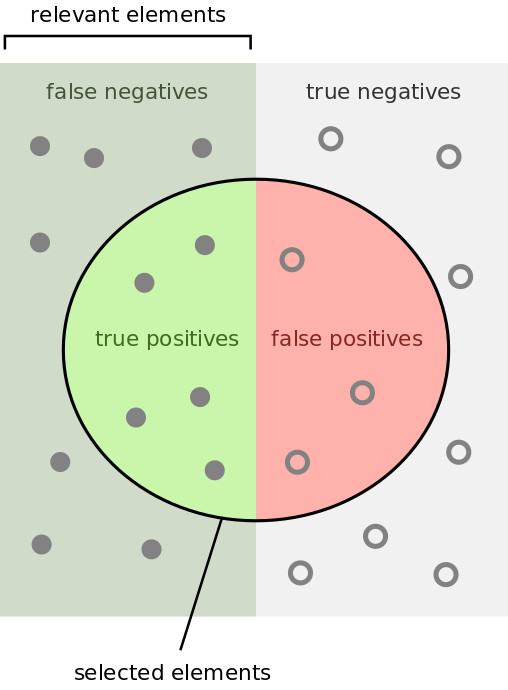
\includegraphics[height=0.8\textheight]{topics/vergleich/pr.jpg}
}


%%Precision recall
\frame{
	\frametitle{Die Maße: Precision und Recall}
	\begin{columns}[c]
    	\begin{column}{5cm}
     		Wie viele der gelieferten Muster sind relevant?
     		$$Precision = \frac{|TP|}{|TP|+|FP|}$$
     		Wie viele der richtigen Muster wurden geliefert? 
     		$$ Recall\frac{|TP|}{|TP|+|FN|}$$
     	\end{column}
    	\begin{column}{5cm}
     		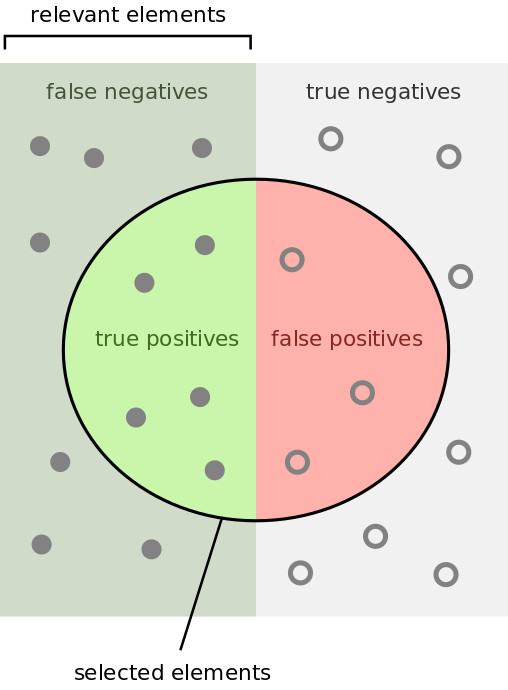
\includegraphics[height=0.8\textheight]{topics/vergleich/pr.jpg}
    	\end{column}
    \end{columns}
}

\frame{
	\frametitle{Ergebnis: Versuch 1}
	\centering
	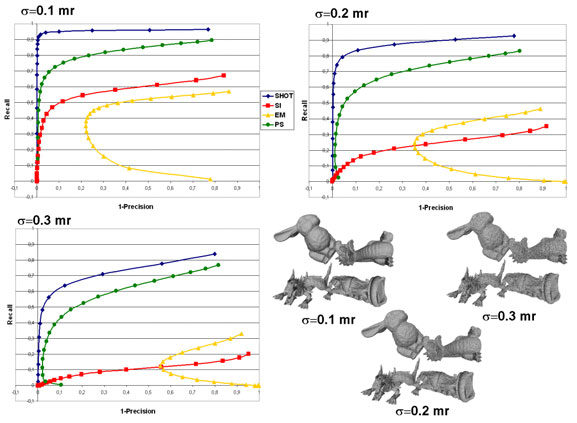
\includegraphics[height=0.8\textheight]{topics/vergleich/v1.png}
}

\frame{
	\frametitle{Ergebnis: Versuch 2}
	\centering
	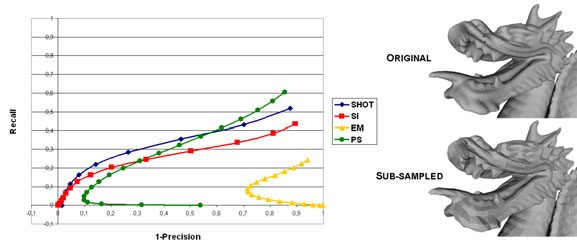
\includegraphics[width=\textwidth]{topics/vergleich/subSampled.png}
}

\frame{
	\frametitle{Ergebnis: Versuch 3}
	\centering
	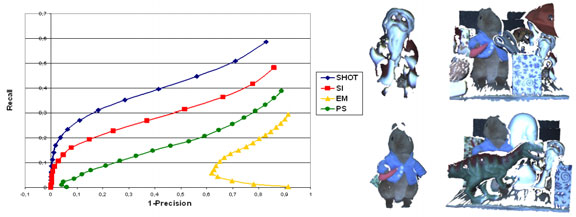
\includegraphics[width=\textwidth]{topics/vergleich/v3.png}
}